\subsubsection{DNA replication}
See illustration how the cell chromosome is used. Some more information may be needed TBD.
When a chromosome is fully duplicated (when the first column of the cell chromosome only contains -2), the process consists of deleting the current chromosome and creating 2 new ones with the correct initialization. TBD do we clean the chromosomes? Typically, when the chromosome was manipulated.

Needs also other things but from the DNA point of view, there seems to have enough information.

\subsubsection{DNA movement}
\textcolor[rgb]{1.00,0.00,0.00}{What do we do when a gene change of volume due to condensation or segregation for example. Normally, a matter of changing the number of the volume in the cell chromosome and the corresponding volume chromosomes. But assume that anything that is currently binded to the DNA is the property of the DNA and was 'erased' from everywhere else. Also assume that volume chromosome only contains the strictly necessary information about the DNA in the volume and that it is a state with changing size.}

\subsubsection{DNA manipulations}
\paragraph{Codon aggregation damage}
\textcolor[rgb]{1.00,0.00,0.00}{Gap site, Abasic site, Sugar-phosphate, Base, Intrastrand cross link, Strand break, Holliday junction}
DNA is subject to numerous forms of damage that can be either endogenous or exogenous. They can result in chemical modifications of some bases, in single strand breakage (missing of one base on one of the strands), double strand breakage or cross links between DNA strands. Chemical modifications can originate from different type of radiations (UV, x-rays, etc.), drugs or reactants naturally present in the cell leading to alkylations, oxydations, deaminations, etc. Another important source of DNA mismatches is the replication machinery itself which can make use of the wrong dNTP (dUTP for example).

DNA modification is one of the prerequisites to evolution. DNA mutations lead to the development of novel functions, regulatory systems, etc. However, replication fidelity is also essential for selection and conservation of important existent functions. There is a trade-off between these two aspects that is well illustrated in \textit{B. subtilis} by the existence of efficient repair mechanism on the one hand and some DNA polymerases that favor propagation of some types of damage (such as DnaE) on the other hand.



\paragraph{Codon aggregation insertion}
Insertion of one (or several) lines in the DNA states.

\paragraph{Codon aggregation deletion}
Putting 0 in the corresponding places and not deletion of the line(s) because a codon aggregation can be deleted in a fork.

\paragraph{Codon aggregation repair}
There are several pathways employed for DNA repair corresponding to the type of damage undergone.

\subparagraph{Mismatch Repair (MMR)} This pathway is dedicated to reparation of base mismatches. In \textit{E. coli}, repairing is initiated by MutS (Sensor) which detects the mismatch and MutL (Linker) which recruits further proteins. The endonuclease MutH then nicks the DNA next to the mismatch enabling the helicase and exonuclase UvrD to remove bases around the mismatch. The resulting gap is filled in by DNA polymerase III and DNA Ligase. The newly synthesized strand is specifically targeted by these proteins thanks to the methylase Dam used for marking the original strand. In \textit{B. subtilis}, only MutS and MutL seem to be conserved (MutL having an additional endonuclease activity). Recognition of the newly synthesized strand could be linked to a strong coupling of MMR with replication and colocalization with the replisome.

\subparagraph{Base excision repair (BER)} The BER pathway repairs most non-bulky base modifications such as oxydations, deaminations, UTP incorporation, etc. Schematically, glycosylases detect the lesion, remove the damaged base, endonucleases then nick the DNA next to the missing base so that exonucleases remove some bases on the strand around the missing base. The small gap is then closed by a repair DNA polymerase (such as Polymerase I) and ligated by a DNA ligase. For example, in \textit{B. subtilis}, the glycosylases MutM and MutY (part of the GO system) detect oxidized Guanine to avoid its pairing up with dATP. Another example is Uracil DNA-glycosylase, which removes dUMP from DNA. 

\subparagraph{Nucleotide excision repair (NER)} The NER pathway is very similar to the BER pathway, except that it repairs bulky lesions caused by UV radiations or drugs. This pathway is highly conserved and partly regulated by the SOS response (mediated by RecA). The UvrABC complex is responsible for detecting the damaged base and nicking the DNA at surrounding bases. Helicase UvrD removes the nicked segment. Finally, DNA Pol. I and DNA ligase restore the missing segment.

\subparagraph{Alkylation damage} There are specific pathways that address alkylation (such as methylations). \textit{B. subtilis}, as a soil-living bacterium, is particularly exposed to alkylating agents. There are at least three pathways responsible for repairing alkylated bases: two pathways based on glycosylases (one being constitutive, the other inducible) and one pathway based on alkyltransferases (enzymes that suicide by transferring the alkyl group onto themselves).

\subparagraph{Homologous recombination (HR)} During replication, double strand breaks (DSB) can be repaired by using the other copy of the chromosome (Figure \ref{fig:HR}). First, the DSB is stabilized by RecN and digested by protein complexes (AddAB and RecQSJ in \textit{B. subtilis}) that create hangovers of single stranded DNA (ssDNA) on the 3' strands. RecA binds to the ssDNA (probably with the help of the RecFOR complex that prevents SSB from binding). RecA, activated by ATP or dATP, enables invasion of the sister chromosome at a homologous sequence, creating a D-loop where one of the broken 3' strands is inserted and forming Holliday Junctions between the two chromosomes. DNA elongation occurs from the 3' strand and the Holliday Junctions are cleaved by RecU (or a homologous protein).

There is a variation if the DSB caused the replication to stall (Figure \ref{fig:HR}, right). This situation may occur if a single-strand break is present on the original chromosome which becomes a DSB after passage of the replication fork. In this case, there is only one DNA end to digest and the invasion leads to only one Holliday Junction. The primosome complex, composed of Pri and Dna proteins, detects the D-loop and helps loading the replisome to resume replication. It seems that several Structural Maintenance of Chromosome (SMC) proteins are involved throughout the process (such as RecN), but their role is not clearly elucidated.

\begin{figure}[!ht]
\centering
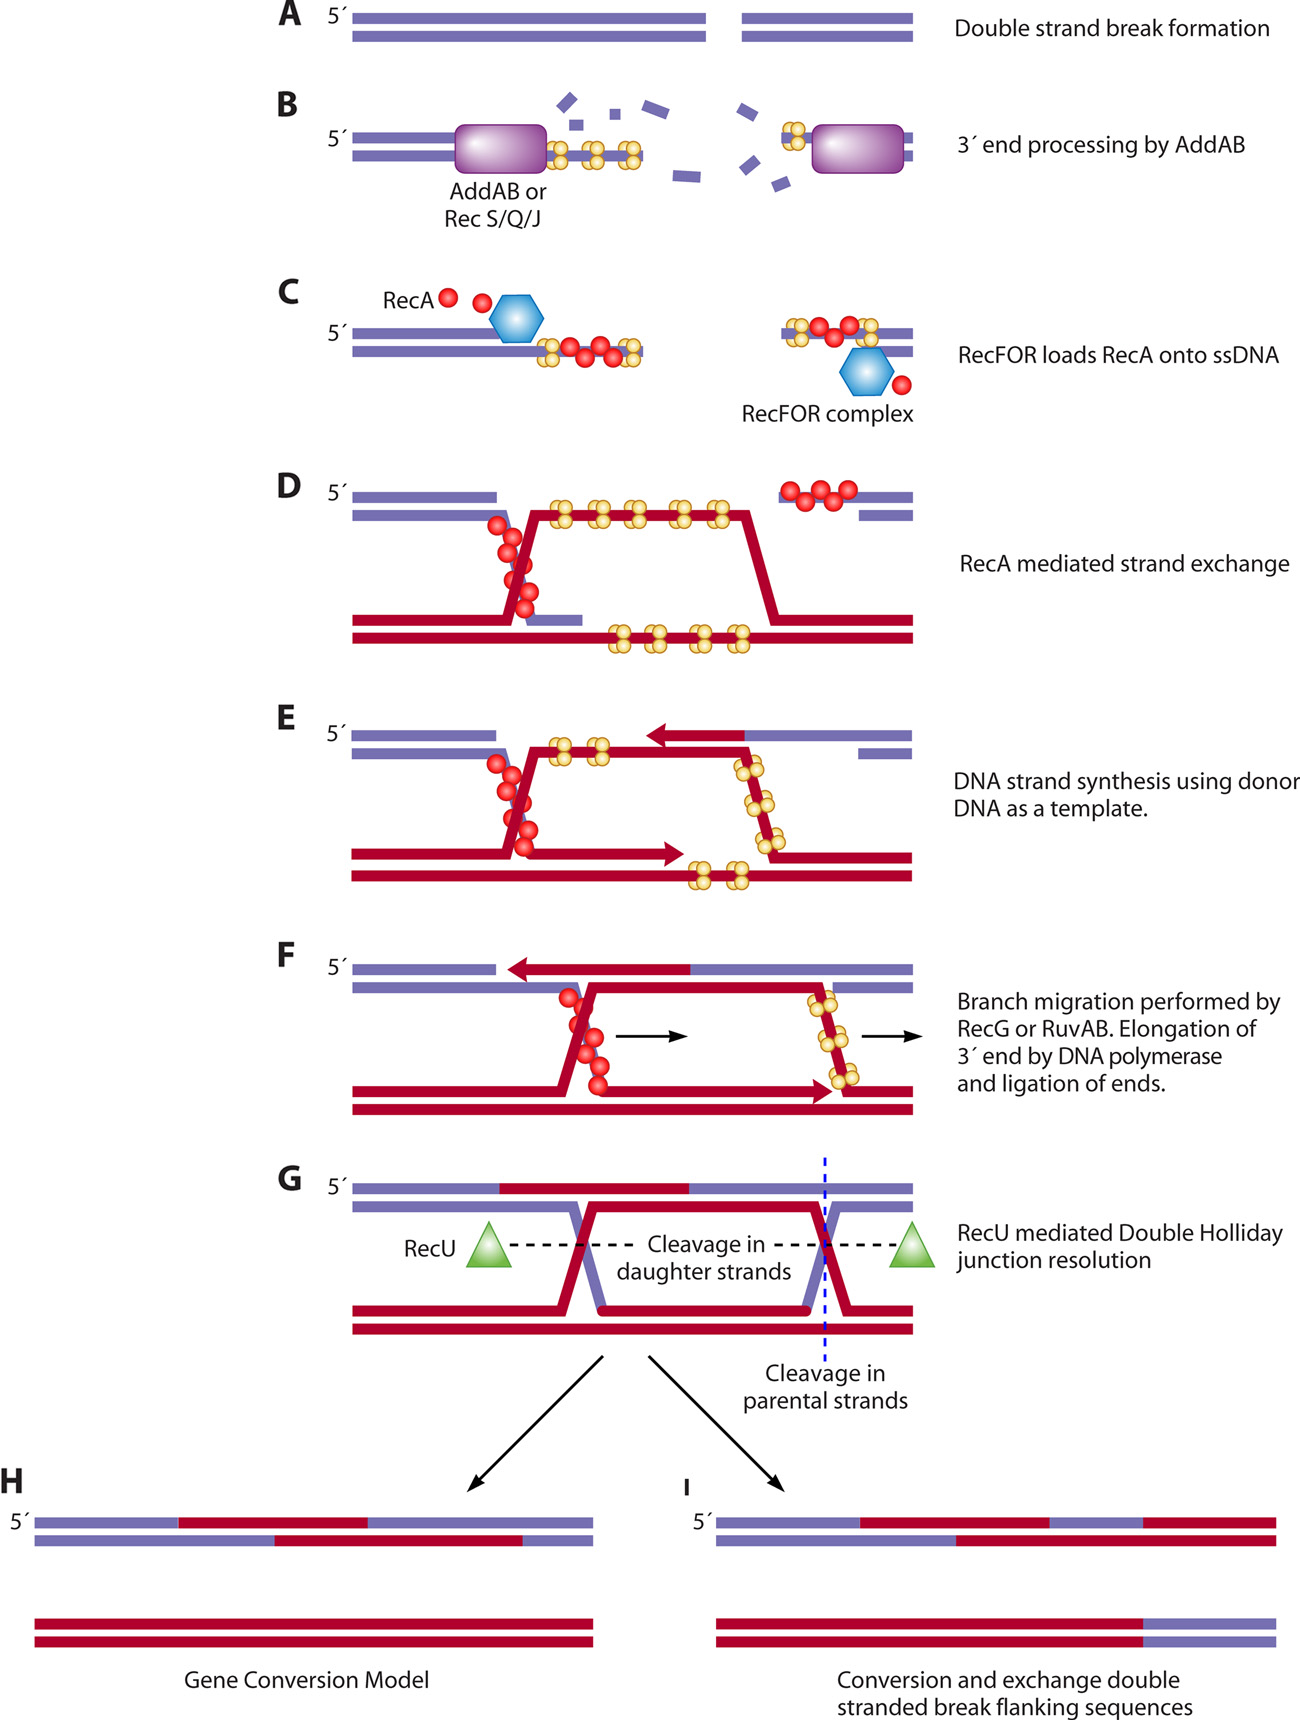
\includegraphics[width=0.54\linewidth]{figure/HR1}
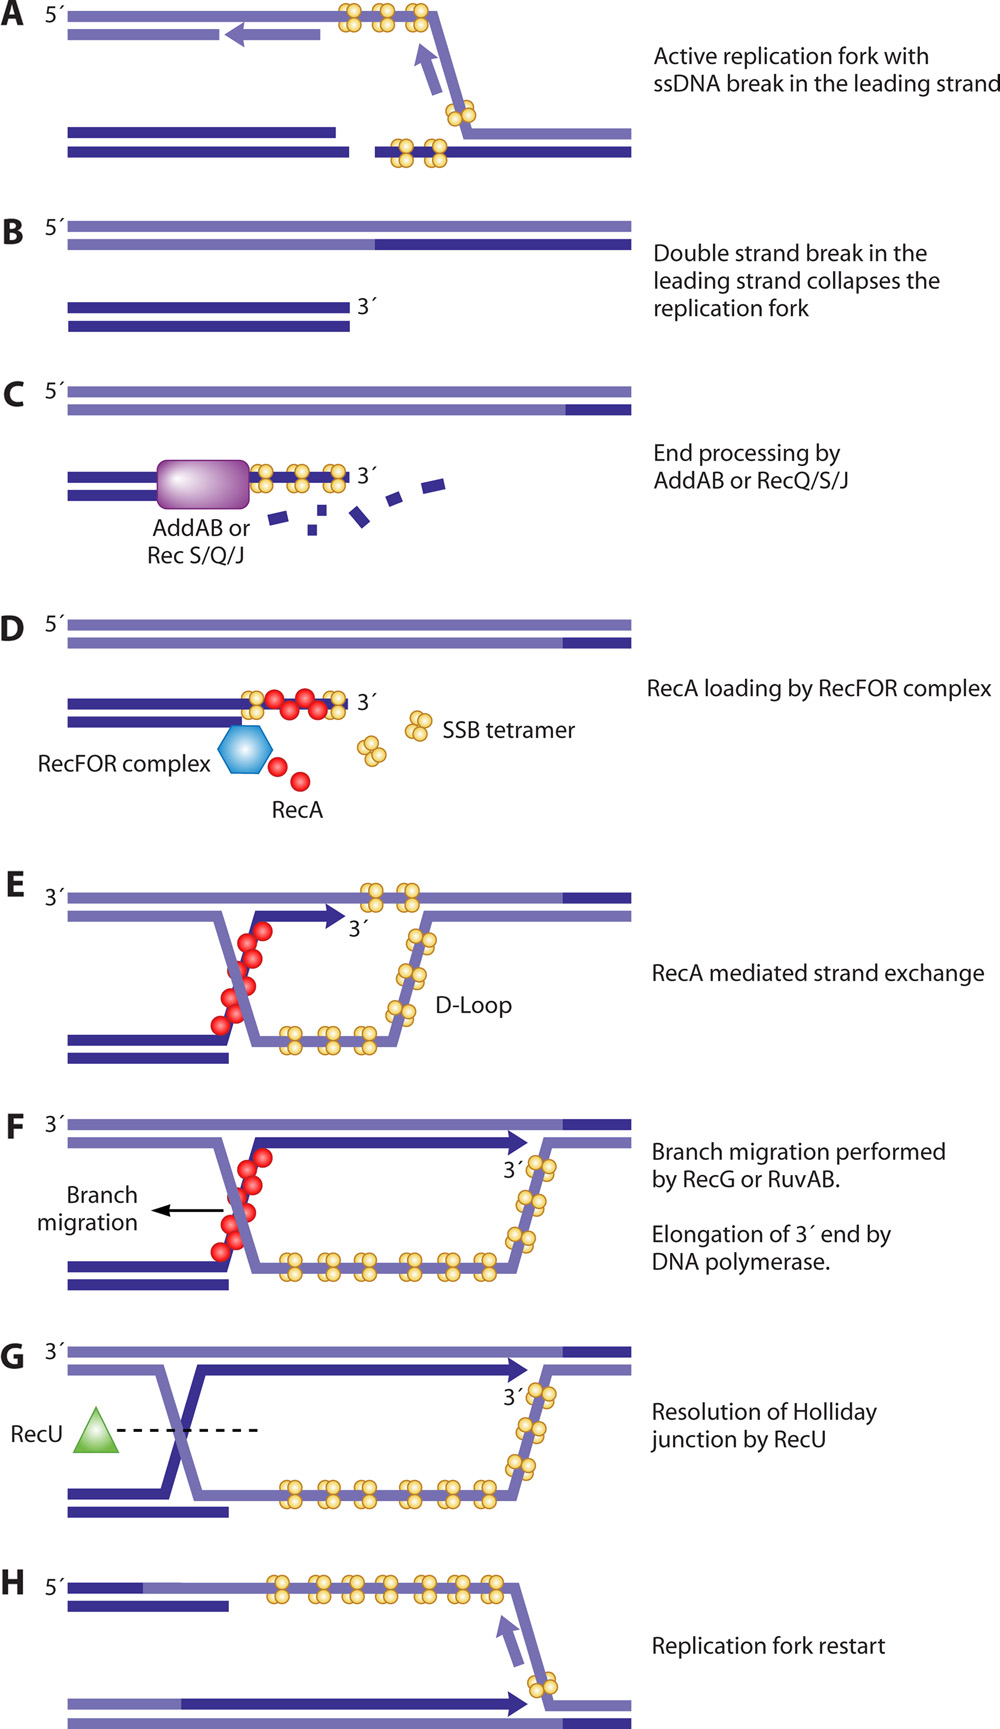
\includegraphics[width=0.44\linewidth]{figure/HR2}
\caption{Homologous recombination and repair of DSB in \textit{B. subtilis} in the general case (left) and when the DSB appears in the replication fork (right). From Lenhart \textit{et al.}.}
\label{fig:HR}
\end{figure}

\subparagraph{Nonhomologous end joining (NHEJ)} This pathway is also responsible for DSB repairing but it is less efficient than homologous recombination. It is used when there is no other copy of the chromosome present in the cell. As in HR, a protein (probably YkoV for \textit{B. subtilis}) binds the DSB and favors recruitment of another protein (LigD like, probably YkoU for \textit{B. subtilis}) that is able to perform exonucleation, polymerisation and ligation. The mechanisms are not totally clear but it seems that because LigD is able to perform these 3 functions, no other protein is needed. However, some bases need to be deleted and repolymerized during the reparation, possibly leading to DNA losses or insertions, making NHEJ a low-fidelity repair mechanism.


\subsubsection{DNA compaction}
\textcolor[rgb]{1.00,0.00,0.00}{Condensation, ”clamping” of the DNA by structural maintenance of chromosome (SMC) proteins, supercoiling, macromolecular crowding, charge neuralization?}
If spatialization is used, condensation and segragation might be modelled directly. Supercoiling needs another state.
\textcolor[rgb]{1.00,0.00,0.00}{Compactation should also impact the accessibility of the chromosome.}

\subsubsection{DNA segregation}
\textcolor[rgb]{1.00,0.00,0.00}{How?}
 

\subsubsection{DNA transformation}

\textcolor{red}{What processes are involved?}
\textcolor{red}{What about plasmid integration, exchange and replication???}
